\chapter{Decomposition Model}

The decomposition model describes the quality attributes of good service decomposition solutions and the criteria leading to such. This chapter starts with an overview over all defined coupling criteria and concludes with the definition of a good decomposition solution. 

\section{Coupling Criteria}
\label{sec:couplingCriteria}

A coupling criterion describes a reason why two nanoentities should or should not be owned by the same service. These criteria define the semantic model on which the Service Cutter is built on. 

The coupling criteria in this thesis are a product of literature research and a workshop assembling the collective software architect experience of our thesis advisor Prof. Dr. O. Zimmermann, our industry partner W. Giersche, a seasoned architect of Zühlke Engineering, and us. we transformed the resulting ideas into the following structured catalog.

\subsection{Criteria Catalog Overview}

The coupling criteria can be classified in a grid as shown in Figure \ref{fig:cc_grid}.

\begin{figure}[H]
	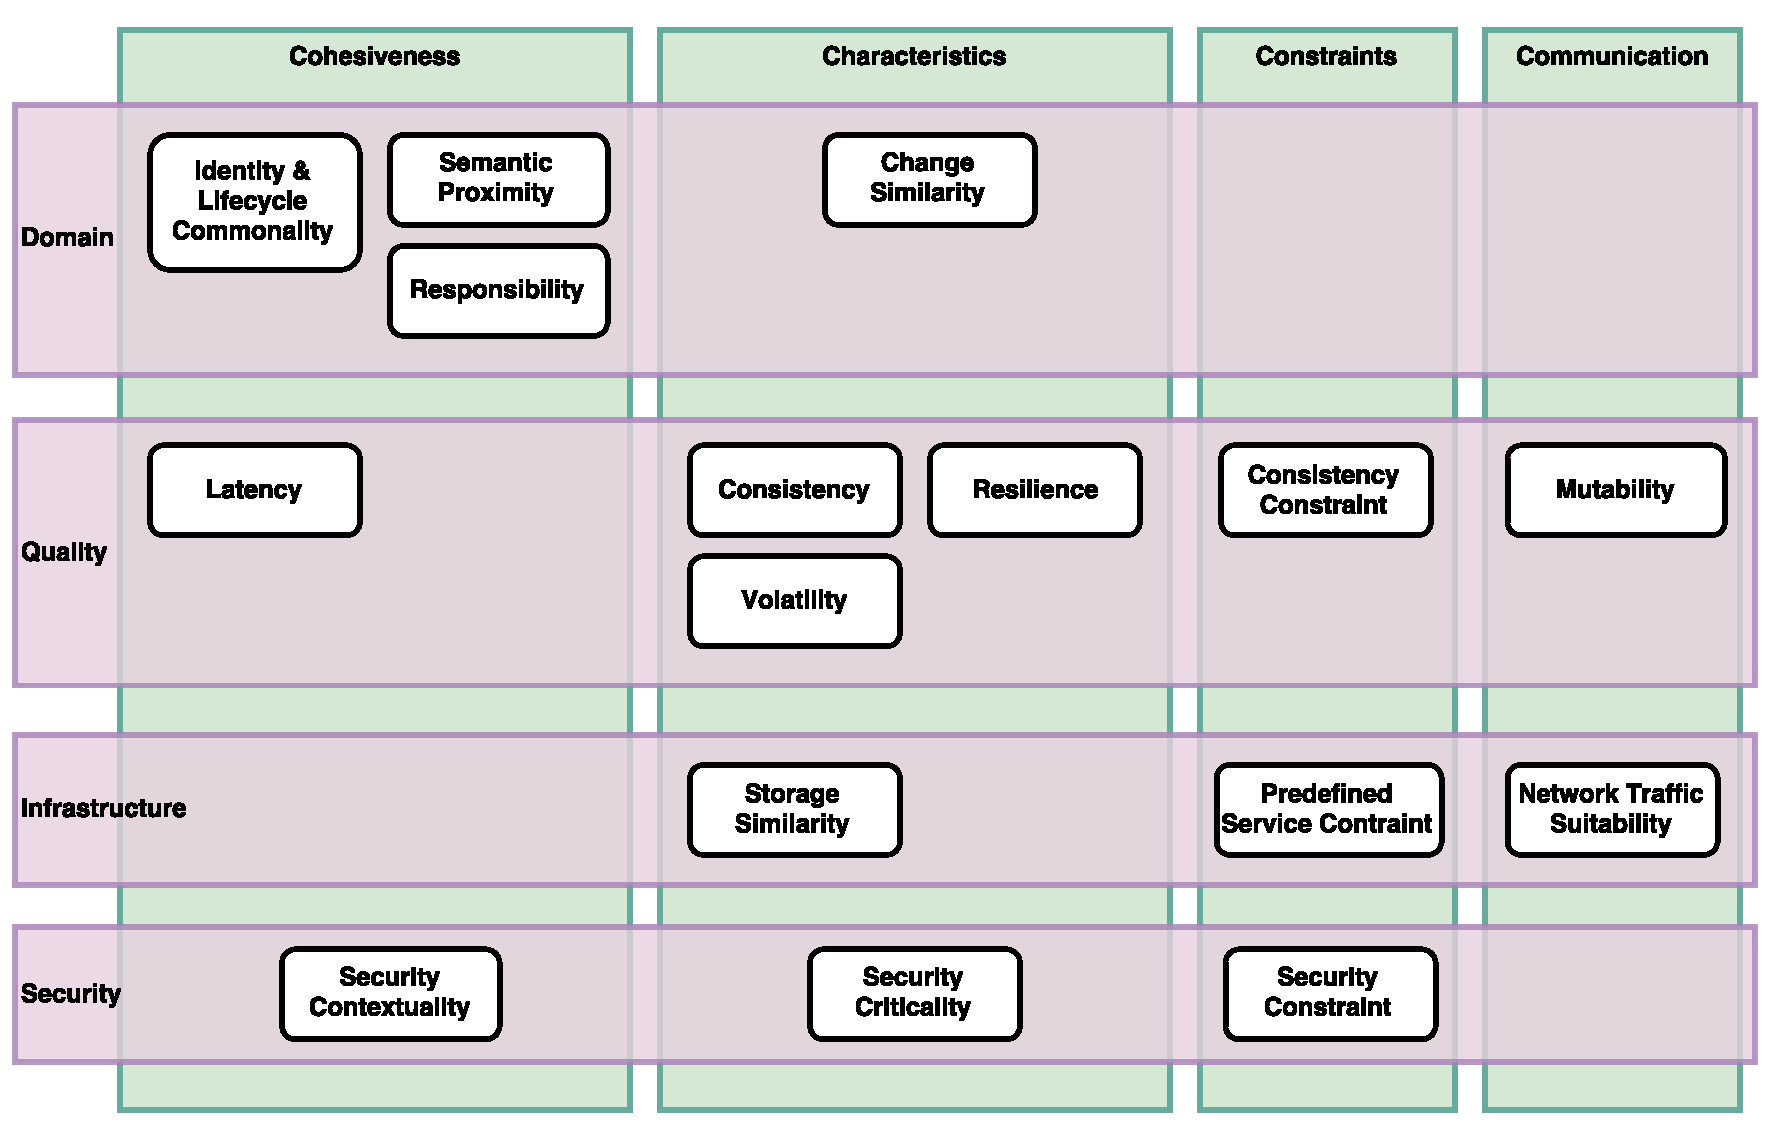
\includegraphics[scale=0.5]{diagrams/CouplingCatalog.pdf}
	\caption{Coupling criteria grid}
	\label{fig:cc_grid}
\end{figure}

The grid columns and rows represent the following partitions:

\begin{description}
	\item[Cohesiveness] - Criteria describing the cohesivness of nanoentities and  therefore why they should belong to the same service. 
	\item[Compatibility] - Criteria describing the incompatible characteristics of nanoentities. The service should not contain nanoentities with different characteristics. Examples for incompatible characteristics are \enquote{High}, \enquote{Eventually}, and \enquote{Weak} for the criterion \enquote{Consistency}.
	\item[Constraints] - Criteria describing constraints which enforce that group of nanoentities must be distributed amongst different services or form a service by itself. (No entities are assigned to another service; no entities are added to this service.)
	\item[Communication] - Criteria describing which nanoentities are suitable to be used as part of the published language shared between services. 
	\item[Domain] Criteria describing nanoentities from a business domain perspective.
	\item[Quality] Criteria describing the quality of service requirements of a nanoentity.  
	\item[Infrastructure] Criteria describing the infrastructural or technological aspects of nanoentities.
	\item[Security] Criteria describing nanoentities from a security perspective.

\end{description}

\subsection{CC Cards}

We specified all coupling criteria listed in the grid as \enquote{CC cards} like the following:

\newcommand{\ccCard}[8] {
\begin{minipage}{\linewidth}
	\begin{framed}
	\textbf{#1 #2}
	
		\begin{description}[leftmargin=!,labelwidth=\widthof{\bfseries User Representation}]
		\item[Description] #3
		\item[User Representation] #4 %TODO source?
		\ifthenelse{\equal{#5}{}}{}{\item[Literature] #5}
		\item[Type] #6
		\item[Perspective] #7
		%\ifx #8\empty  #8 \fi
		\ifthenelse{\equal{#8}{}}{}{\item[Characteristics] #8}
		\end{description}
	
	\end{framed}
\end{minipage}
}
\ccCard{CC-1}{Identity \& Lifecycle Commonality}{Nanoentities that belong to the same identity and therefore share a common lifecycle. }{- UML class diagrams (Same Class, Composition, Inheritance) \newline - Domain-Driven Design entities.}{Entity definition in Domain-Driven Design: \newline \textit{Some objects are not defined primarily by their attributes. They represent a thread of identity that	runs through time and often across distinct representations.}\cite{evans2003domain}}{Cohesiveness}{Domain}{}


Cards share the following information:

\begin{description}
	\item[Description] Explains the coupling criteria in more detail.
	\item[User Representation] Lists familiar concepts that can be used to feed the criteria information into the Service Cutter.
	\item[Literature] References the coupling criteria to descriptions in existing literature.
	\item[Type] The type of the criterion: Cohesiveness, Compatibility, Constraint or Communication.
	\item[Perspective] The perspective of the criterion: Domain, Quality, Infrastructure or Security. 
	\item[Characteristics] Cards of type \enquote{compatibility} list different characteristics that can be applied to a nanoentity.
\end{description}

\ccCard{CC-2}{Semantic Proximity}{Two nanoentities are semantically proximate when they have a semantic connection given by the business domain. The strongest indicator for semantic proximity is coherent access on nanoentities within the same use case.}{- Coherent access or updates on nanoentities in use cases.\newline - Aggregation or association relationships in UML class diagrams.}{Chris Richardson on microservice decomposition:\newline \textit{Deciding how to partition a system into a set of services is very much an art but there are number of strategies that can help. One approach is to partition services by verb or use case.}\cite{microserviceIntro}\newline Single Responsibility Principle by C. Martin:\newline \textit{Gather together the things that change for the same reasons. Separate those things that change for different reasons.}\cite{SRP}}{Cohesiveness}{Domain}{}
%todo literature based on use case driven services?

\ccCard{CC-3}{Responsibility}{The same person, role or department is responsible for a group of nanoentities. Service decomposition should try to keep entities with the same responsible instance together while not mixing entities with different responsible instances in one service. }{User defined persons, roles or departments with each containing a group of nanoentities. A nanoentity can only be associated once.}{Conway's law:\newline \textit{Organizations which design systems are constrained to produce designs which are copies of the communication structures of these organizations.}\cite{conway}\newline Single Responsibility Principle by C. Martin:\newline \textit{Gather together the things that change for the same reasons. Separate those things that change for different reasons. [...] However, as you think about this principle, remember that the reasons for change are people. It is people who request changes. And you don't want to confuse those people, or yourself, by mixing together the code that many different people care about for different reasons.}\cite{SRP}}{Cohesiveness}{Domain}{}

\ccCard{CC-4}{Change Similarity}{How often change requests need to be implemented affecting nanoentities.}{Classification of nanoentities in characteristics.}{David L. Parnas on modular programming: \newline \textit{We propose instead that one begins with a list of difficult design decisions or design decisions which are likely to change. Each module is then designed to hide such a decision from the others.}\cite{parnaDecomposing}}{Compatibility}{Domain}{Often, Normal \textit{(default)}, Rarely}

\ccCard{CC-5}{Latency}{Groups of nanoentities with high performance requirements for a specific user request. These nanoentities should be modelled within the same service to avoid remote calls.}{Use cases with high performance requirements. All nanoentities read or written by the use case belong a group. A nanoentity can belong to multiple groups.}{Design guidelines for application performance by Microsoft: \newline \textit{Minimize round trips to reduce call latency. For example, batch calls together and design coarse-grained services that allow you to perform a single logical operation by using a single round trip.}\cite{performance}}{Cohesiveness}{Quality}{}

\ccCard{CC-6}{Consistency}{Some data loses its value when not kept consistent together while other data is more tolerant to inconsistencies.}{Classification of nanoentities in characteristics.}{Werner Vogel on consistency requirements: \newline  
\textit{\textbf{Strong consistency}: After the update completes, any subsequent access (by A, B, or C) will return the updated value. \newline \textbf{Weak consistency}: The system does not guarantee that subsequent accesses will return the updated value. A number of conditions need to be met before the value will be returned. The period between the update and the moment when it is guaranteed that any observer will always see the updated value is dubbed the inconsistency window.}\cite{consistency}}{Compatibility}{Quality}{High consistency \textit{(default)}, eventual consistency, weak consistency}
%TODO: only High & Weak?

\ccCard{CC-7}{Resilience}{Nanoentities have varying availability constraints. Some are critical while others can be unavailable for some time. As providing high availability comes at a cost, nanoentities classified with different characteristics should not be composed in the same service.}{Classification of nanoentities in characteristics.}{E. Woods on availability and resilience: \newline \textit{Getting your availability characteristics wrong can be very expensive. However, increased online availability comes at a cost, whether in terms of more hardware, increased software sophistication, or redundancy in your communications network.}\cite{rozanski2011software} }{Compatibility}{Quality}{Critical, Normal \textit{(default)}, Low}

\ccCard{CC-8}{Volatility}{A nanoentity can be classified by its volatility which defines how frequent it is updated. Highly volatile and more stable nanoentities should be composed in different services.}{- Volatility can be calculated from use case definitions if they are equipped with a frequency information. \newline- Nanoentities can be classified by data types to determine the volatility: Master Data (regularly), Reference Data (rarely), Transaction Data (often) and Inventory Data (often) to determine the volatility.}{}{Compatibility}{Quality}{Often, Regularly \textit{(default)}, Rarely}
%TODO add literature (datentypen?)

\ccCard{CC-9}{Consistency Constraint}{A group of nanoentities that have a dependent state and therefore need to be kept consistent to each other. }{An aggregate as defined in domain-driven design.}{Aggregate as defined in domain-driven design by E. Evans: \newline \textit{A cluster of associated objects that are treated as a unit for the purpose of data changes. External references are restricted to one member of the aggregate, designated as the root. A set of consistency rules applies within the aggregate's boundaries.}\cite{evans2003domain} \newline Udi Dahan on service decomposition: \newline \textit{If modifying the value of one attribute involves changing the value of another, then those two attributes should fall under the responsibility of the same service.}\cite{udiConsistency}}{Constraint}{Quality}{}


\ccCard{CC-10}{Mutability}{Immutable information is much simpler to manage in a distributed system than mutable objects. Immutable nanoentities are therefore good candidates for the published language shared between two services. Service decomposition should be done in a way that favors sharing immutable nanoentities over mutable ones. }{Classification of each nanoentity in mutable or immutable.}{Udi Dahan on finding service boundaries:\newline \textit{When you find something immutable, that is an indication that there is some loose coupling between the two sides passing immutable data.}\cite{mutability}}{Communication}{Quality}{}

\ccCard{CC-11}{Storage Similarity}{Storage that is required to persist all instances of a nanoentity.}{The user classifies nanoentities into the given characteristics. The classification is system specific. In one system a nanoentity classified as \textit{huge} might need 1MB, but in another 1GB storage per instance.}{}{Compatibility}{Infrastructure}{Huge, Normal \textit{(default)}, Tiny}

\ccCard{CC-12}{Predefined Service Constraint}{There might be the following reasons why some nanoentities forcefully need to be modelled in the same service: \newline - Technological optimizations \newline - Legacy systems}{User defined service with each containing a group of nanoentities. Each nanoentity can be associated only once.}{}{Constraint}{Infrastructure}{}

\ccCard{CC-13}{Network Traffic Similarity}{Service decomposition has a significant impact on network traffic, depending on which nanoentities are shared between services and how often. Small and less frequently accessed nanoentities are better suited to be shared between services.}{Use cases define the frequency of access on nanoentities. The size of each entity can be determined by CC-11: Storage Similarty}{}{Communication}{Infrastructure}{}

\ccCard{CC-14}{Security Contextuality}{A security role is allowed to see or process a group of nanoentities. Mixing security contexts in one service complicates authentication and authorization implementations.}{User defined security roles with each containing a group of nanoentities. A nanoentity can be associated to multiple groups.}{}{Cohesiveness}{Security}{}

\ccCard{CC-15}{Security Criticality}{Criticality of an nanoentity in case of data loss or a privacy violation. Represents the reputational or financial damage when the information is disclosed to unauthorized parties. As high security criticality comes at a cost, nanoentities classified with different characteristics should not be composed in the same service. }{Classification of nanoentities in characteristics}{}{Compatibility}{Security}{Critical, Internal \textit{(default)}, Public}

\ccCard{CC-16}{Security Constraint}{Groups of nanoentities are semantically related but must not reside in the same service in order to satisfy information security requirements. This restriction can be established by an external party such as a certification authority or an internal design team.}{Demilitarized zones or other groups of nanoentities that should be composed to different services.}{}{Constraint}{Security}{}



% \ccCard{CC-}{}{}{}{}{}{}


\section{What is a good Decomposition Solution?}
\label{sec:decompositionRequirements}

Based on the coupling criteria described above and to achieve the principles introduced in Chapter \ref{cha:analysis}, we define a good decomposition solution as following:

\begin{enumerate}
	\item Not violating any constraints criteria.
	\item Combining as few nanoentities with different characteristics in one service as possible.
	\item Each service should depend on as few nanoentities of other services as possible (A use case should cross as few service boundaries as possible).
	\item Nanoentities which are part of a published language between services should be suitable for inter service communication (Network Traffic Suitability, Mutability).
	\item The coupling a single service has to other services should be similar for all services. It is not the size of services that requires homogeneity within the system but the amount of published language  each service shares. 
	\item Not too many services which leads to the nanoservice antipattern\cite{nanoservice}.
	\item Not too few services, which leads to a monolithic architecture.
\end{enumerate}



%TODO User stories as most important criteria: check Ivar Jacobson, oose, a use case driven approach

%TODO: Should we describe non relevant coupling criteria as well? (Hiding design decisions etc, see CC catalog doc)

%TODO: (Bring result \& discussion already here?)
